\documentclass[pdflatex,sn-mathphys-num]{sn-jnl}% Math and Physical Sciences Numbered Reference Style

\usepackage{graphicx}%
\usepackage{multirow}%
\usepackage{amsmath,amssymb,amsfonts}%
\usepackage{amsthm}%
\usepackage[title]{appendix}%
\usepackage{xcolor}%
\usepackage{textcomp}%
\usepackage{manyfoot}%
\usepackage{booktabs}%
\usepackage{algorithm}%
\usepackage{algorithmicx}%
\usepackage{algpseudocode}%
\usepackage{listings}%

\providecommand{\code}[1]{\texttt{#1}}%
\algrenewcommand\algorithmicrequire{\textbf{Input:}}
\algrenewcommand\algorithmicensure{\textbf{Output:}}

\theoremstyle{thmstyleone}%
\newtheorem{theorem}{Theorem}%
\newtheorem{proposition}[theorem]{Proposition}%

\theoremstyle{thmstyletwo}%
\newtheorem{example}{Example}%
\newtheorem{remark}{Remark}%

\theoremstyle{thmstylethree}%
\newtheorem{definition}{Definition}%

\raggedbottom

\begin{document}
\graphicspath{{figures/}}

\title[Adaptive Identification and Tracking]{Adaptive Candidate Routing for Distributed Occupant Recognition Across Multiple Building IoT-enabled Smart Spaces}

\author*[1,2]{\fnm{First} \sur{Author}}\email{iauthor@gmail.com}

\author[2,3]{\fnm{Second} \sur{Author}}\email{iiauthor@gmail.com}
\equalcont{These authors contributed equally to this work.}

\author[1,2]{\fnm{Third} \sur{Author}}\email{iiiauthor@gmail.com}
\equalcont{These authors contributed equally to this work.}

\affil*[1]{\orgdiv{Department}, \orgname{Organization}, \orgaddress{\street{Street}, \city{City}, \postcode{100190}, \state{State}, \country{Country}}}

\affil[2]{\orgdiv{Department}, \orgname{Organization}, \orgaddress{\street{Street}, \city{City}, \postcode{10587}, \state{State}, \country{Country}}}

\affil[3]{\orgdiv{Department}, \orgname{Organization}, \orgaddress{\street{Street}, \city{City}, \postcode{610101}, \state{State}, \country{Country}}}


\abstract{This work proposes a multi-building biometric-embedding routing mechanism for occupant identification and tracking across indoor environments in IoT-enabled smart spaces. Centralized galleries raise privacy concerns, while distributed galleries incur overhead in locating the appropriate building before recognition. The proposed approach models the environment using a Distributed State Transition System (DSTS), where states represent occupant presence probabilities, events represent biometric recognition, and transitions describe state evolution. Each building shares a Bloom filter constructed from locality-sensitive hashing (LSH) codes of its registered occupants. A captured face generates $L$ codes, which are checked against all filters to rank candidate buildings. Only the highest-ranked buildings verify the face against their reference embeddings. Experiments involving 500 CASIA-WebFace identities across 10 buildings, averaged over 20 random assignments, achieve 92.81\% correct identification for routed visitors, compared with 95.50\% for centralized recognition. An adaptive strategy querying additional buildings when rankings are ambiguous achieves 92.95\% for routed visitors while contacting an average of 2.54 buildings per query. The filter false-positive rate is 3.54\%, exceeding the configured 1\% because of LSH code collisions. Communication payload is estimated rather than measured, and encryption and unknown visitors remain unevaluated.}
\keywords{Occupant identification and tracking, Distributed state transition system, Smart spaces, Locality-sensitive hashing, Bloom filter, Face recognition}


\maketitle


\section{Introduction}

Camera networks are widely deployed across IoT-enabled smart spaces to monitor occupants and support occupant-specific building-level services~\cite{SM2022,hou2017}. These applications require reliable occupant identification and tracking to associate facial observations with the correct individuals. When such services span multiple buildings, identity resolution depends on how biometric reference data are maintained and accessed across the buildings. Centralized architectures maintain a common database of reference face embeddings, whereas distributed architectures retain biometric reference data within individual buildings. Centralized approaches concentrate sensitive biometric data in one location and introduce a potential single point of failure. Although distributed architectures reduce dependence on a central repository, they introduce challenges in identifying occupants across building boundaries~\cite{mohan2020}.

In a distributed setting, an individual registered with one building may be treated as a visitor upon entering another building where the individual is not registered. Identifying such visitors is challenging because the potential visitor set of a building may include occupants registered across other buildings and may approach the size of the overall registered population. Supporting visitor identification may require reference embeddings to be shared across buildings or multiple local galleries to be searched, increasing computational overhead and potentially exposing additional biometric data.


To address this challenge, this work proposes a decentralized face recognition strategy that uses locality-sensitive hashing (LSH) and Bloom filters to route query embeddings to candidate buildings while retaining reference embeddings locally. Each building-level state transition system (BSTS) shares a Bloom filter constructed from the LSH codes of its registered occupants' face embeddings with all other buildings. Query embeddings are used to rank candidate BSTSs, and local angular-distance voting verifies identity only at the selected buildings. The framework is evaluated using 500 CASIA-WebFace identities across ten simulated buildings, with results averaged over 20 random assignments. The adaptive policy achieves 92.95\% correct identification while contacting an average of 2.54 buildings per query, compared with 95.50\% for centralized search.

The remainder of this paper is organized as follows. Section~\ref{sec:related} reviews related work on occupant identification, distributed state transition systems, biometric privacy, and distributed query routing. Section~\ref{sec:methodology} describes the proposed framework, including LSH encoding, Bloom-filter construction, candidate routing, and local verification. Section~\ref{sec:setup} presents the experimental setup and evaluation metrics. Section~\ref{sec:results} reports the experimental results, followed by a discussion in Section~\ref{sec:discussion}. Section~\ref{sec:conclusion} concludes the paper and outlines future research directions, while Section~\ref{sec:limitations} summarizes the limitations of the current evaluation.



%=====================================================================
\section{Related Work}
\label{sec:related}

Occupant identification and tracking in IoT-enabled smart spaces rely on camera-based and radio-frequency (RF)-based sensing~\cite{mohan2020,WZSYGWLLHSC2025}, and Wi-Fi-based indoor localization uses weighted trilateration over dual-band signals~\cite{MSSAB2019}. Camera-based systems enable unobtrusive facial identification, including tracking across non-overlapping cameras~\cite{nair2021}. In multi-building deployments, identity verification that depends on a central store of biometric data raises computational and privacy concerns~\cite{mohan2020}.

State transition models represent occupant tracking through states, recognition events, and transition functions~\cite{MJG2011}. The DSTS extends this approach to multiple buildings, each represented by a BSTS, where registered occupants are recognized against the local database of their building and visitors are resolved through a centralized master list~\cite{mohan2020}. Related work also addresses video synopsis~\cite{NGA2022} and quantitative metrics for smart spaces~\cite{MMJ2025}. Privacy-preserving biometric methods include Bloom-filter protection of iris templates~\cite{rathgeb2014}, and Marzani et al.~\cite{marzani2026} combine face features, fuzzy extractors, and homomorphically encrypted Bloom filters to count individuals across locations. In contrast, the present work uses LSH codes and per-BSTS Bloom filters to route a captured embedding towards candidate buildings on the basis of approximate similarity, while the reference embeddings remain local.

The proposed routing builds on established techniques. Random-hyperplane LSH preserves angular similarity in binary codes~\cite{charikar2002}, and multi-probe lookup examines nearby codes to improve recall without additional hash tables~\cite{lv2007}. Bloom filters~\cite{bloom1970} provide compact approximate set membership, with filter positions derived by double hashing~\cite{kirsch2006}. In distributed search, Summary Cache~\cite{fan2000} uses Bloom filters to identify web proxies likely to hold requested objects, Gottesb{\"u}ren et al.~\cite{gottesbueren2024} study partitioning-based routing of nearest-neighbor search requests to relevant data shards, and Semord~\cite{wang2026semord} organizes similar vectors in a decentralized overlay using learned hashing and exchanged summaries. Unlike approaches that rely on vector placement or shared vector summaries, the proposed framework shares only compact Bloom filters of LSH codes and does not distribute reference face embeddings. To the best of our knowledge, this combination has not previously been evaluated for occupant identification across multiple BSTSs.

% ============================================================
% METHODOLOGY
% ============================================================

\section{Methodology}
\label{sec:methodology}

\subsection{System Model and Assumptions}
\label{subsec:system_model}

This work addresses the visitor identification step of the DSTS framework of Mohan and Menon~\cite{mohan2020}. In that framework, an occupant registered in a building is recognized by comparison with the local database of that building, whereas visitors are resolved through a centralized master list. The contribution is a candidate-routing and visitor-identification component for a DSTS-based architecture: an accepted identity is supplied to the DSTS as a recognition event, and the state and transition models are neither implemented nor evaluated here. The sub-problem considered is identifying a visitor, that is, an individual observed in a building where the individual is not registered and whose reference embeddings are held by another building. The aim is to locate that building and verify the visitor there without matching the captured embedding against the reference embeddings of every building.

The environment consists of $B$ buildings, each with a BSTS that maintains a local reference database $\mathcal{D}_b$, $b\in\{1,\ldots,B\}$, containing the reference face embeddings of its registered occupants. Each BSTS builds a Bloom filter from the LSH codes of its registered occupants and shares it with all other BSTSs, so that every building holds the filters of all $B$ buildings while keeping $\mathcal{D}_b$ local. When a face is captured in a building and no occupant of that building accepts it, the captured embedding is checked against the filters of the other buildings, which ranks them and selects a shortlist. The captured embedding is then sent to the shortlisted buildings, which verify it against their local reference embeddings and return the result. The system abstains if none of them accepts. A centralized system that holds all reference embeddings in a single database serves as the performance baseline. Communication between buildings is assumed to be secured by the deployment infrastructure, and encryption is neither implemented nor evaluated. LSH codes and Bloom filters are compact routing representations and not encryption mechanisms, so no formal privacy guarantee is claimed.

\subsection{LSH Encoding}
\label{subsec:lsh_encoding}

Faces are detected and aligned with SCRFD-10GF~\cite{guo2022} and embedded with a pretrained ArcFace model~\cite{deng2019} (InsightFace \code{buffalo\_l}), for reference and captured images alike. A raw embedding $\hat{\mathbf{e}}^{\mathrm{raw}}\in\mathbb{R}^{512}$ is normalized, centered with the reference-derived mean $\bar{\mathbf{x}}$, and normalized again:
\begin{equation}
    \hat{\mathbf{e}}
    =
    \frac{
        \frac{\hat{\mathbf{e}}^{\mathrm{raw}}}{\|\hat{\mathbf{e}}^{\mathrm{raw}}\|_2}
        - \bar{\mathbf{x}}
    }{
        \left\|
        \frac{\hat{\mathbf{e}}^{\mathrm{raw}}}{\|\hat{\mathbf{e}}^{\mathrm{raw}}\|_2}
        - \bar{\mathbf{x}}
        \right\|_2
    }.
    \label{eq:embedding_preprocessing}
\end{equation}
The $R$ preprocessed reference embeddings $\hat{\mathbf{e}}_{u,1},\ldots,\hat{\mathbf{e}}_{u,R}$ of a registered occupant $u$ give a normalized centroid
\begin{equation}
    \mathbf{z}_u
    =
    \frac{
        \sum_{r=1}^{R}\hat{\mathbf{e}}_{u,r}
    }{
        \left\|\sum_{r=1}^{R}\hat{\mathbf{e}}_{u,r}\right\|_2
    },
    \label{eq:identity_centroid}
\end{equation}
and LSH codes are computed from $\mathbf{z}_u$ for registered occupants and from $\hat{\mathbf{e}}$ for captured faces.

The codes use random hyperplanes~\cite{charikar2002}: vectors $\mathbf{w}_{\ell,k}\in\mathbb{R}^{512}$ ($\ell<L$, $k<K$), drawn once from a standard Gaussian distribution and shared by all buildings, define $L$ slots of $K$ bits. The bit $h_{\ell,k}$ records the side of the hyperplane on which the embedding lies, and the $K$ bits of slot $\ell$ form an integer code:
\begin{equation}
    h_{\ell,k}(\hat{\mathbf{e}}) =
    \begin{cases}
        1, & \mathbf{w}_{\ell,k}^\top\hat{\mathbf{e}} \geq 0,\\
        0, & \text{otherwise},
    \end{cases}
    \qquad
    c_\ell(\hat{\mathbf{e}}) = \sum_{k=0}^{K-1} 2^{k}\, h_{\ell,k}(\hat{\mathbf{e}}) \in \{0,\ldots,2^K-1\}.
    \label{eq:lsh_bit}
\end{equation}
Each code is tagged with its slot identifier,
\begin{equation}
    s_\ell(\hat{\mathbf{e}})
    =
    \ell 2^K + c_\ell(\hat{\mathbf{e}}),
    \label{eq:tagged_code}
\end{equation}
so that codes from different slots are never confused; an embedding is represented by $L$ tagged codes (Algorithm~\ref{alg:build}). Embeddings at angle $\theta$ agree on one bit with probability $1-\theta/\pi$~\cite{charikar2002}, on all $K$ bits of a slot with probability $(1-\theta/\pi)^K$, and on at least one of the $L$ slots with probability
\begin{equation}
    P_{\mathrm{match}}(\theta)=1-\Bigl(1-\bigl(1-\tfrac{\theta}{\pi}\bigr)^{K}\Bigr)^{L}.
    \label{eq:slot_agreement}
\end{equation}
$P_{\mathrm{match}}(\theta)$ is high for the small angles of the same person and low for the large angles between different people; a larger $K$ reduces chance agreement and a larger $L$ raises the agreement of the same identity.

\subsection{Bloom-Filter Construction and Sharing}
\label{subsec:bloom_filter}

Each building $b$ inserts the $L$ tagged items of each of its $N$ registered occupants into its Bloom filter $F_b$~\cite{bloom1970}, so $n=N\cdot L$ items are inserted (Algorithm~\ref{alg:build}). A Bloom filter reports an item as absent or as possibly present, so a positive can be false. For a target false-positive probability $f^*$, the filter size $m$ (in bits) and the number of hash positions $\kappa$ are
\begin{equation}
    m =
    \left\lceil
    -\frac{n\ln f^*}{(\ln 2)^2}
    \right\rceil,
    \qquad
    \kappa =
    \operatorname{round}
    \left(\frac{m}{n}\ln 2\right).
    \label{eq:bloom_size}
\end{equation}
The $\kappa$ positions of an item $s$ come from double hashing~\cite{kirsch2006} of two 64-bit hash values and a shared salt, and $\textsc{Insert}(F_b,s)$ sets them in $F_b$. Each building shares its filter with all other buildings; the filters are the only data exchanged in advance, and reference embeddings are not shared. A positive response only qualifies a building as a candidate.

\begin{algorithm}[!t]
\footnotesize
\caption{LSH encoding and Bloom-filter construction at building $b$}
\label{alg:build}
\begin{algorithmic}[1]
\Require Raw reference embeddings $\hat{\mathbf{e}}^{\mathrm{raw}}_{u,r}$ of $N$ occupants ($R$ each), mean $\bar{\mathbf{x}}$, vectors $\mathbf{w}_{\ell,k}$, $K$, $L$ (Section~\ref{subsec:lsh_encoding}), $f^*$ (Section~\ref{subsec:bloom_filter})
\Ensure Bloom filter $F_b$, shared with all other buildings
\State $n\gets N\cdot L$; compute $m$ and $\kappa$ from $n$ and $f^*$ \Comment{Eq.~\eqref{eq:bloom_size}}
\State $F_b\gets$ bit array of $m$ zeros
\For{each registered occupant $u=1,\dots,N$}
  \State $\hat{\mathbf{e}}_{u,r}\gets$ preprocess $\hat{\mathbf{e}}^{\mathrm{raw}}_{u,r}$ for $r=1,\dots,R$ \Comment{Eq.~\eqref{eq:embedding_preprocessing}}
  \State $\mathbf{z}_u\gets$ normalized sum of $\hat{\mathbf{e}}_{u,1},\dots,\hat{\mathbf{e}}_{u,R}$ \Comment{Eq.~\eqref{eq:identity_centroid}}
  \For{each slot $\ell=0,\dots,L-1$}
    \State $h_{\ell,k}\gets[\mathbf{w}_{\ell,k}^\top\mathbf{z}_u\geq 0]$ for $k=0,\dots,K-1$; $c_\ell\gets\sum_{k}2^{k}h_{\ell,k}$ \Comment{Eq.~\eqref{eq:lsh_bit}}
    \State $s_\ell\gets\ell 2^K+c_\ell$; \textsc{Insert}$(F_b,s_\ell)$ \Comment{Eq.~\eqref{eq:tagged_code}; set the $\kappa$ bit positions}
  \EndFor
\EndFor
\State share $F_b$ with all other buildings; \Return $F_b$
\end{algorithmic}
\end{algorithm}

\subsection{Routing and Verification}
\label{subsec:routing_verification}

For a captured embedding, the building where the face is captured computes the $L$ tagged codes of Eq.~\eqref{eq:tagged_code} and checks them against the Bloom filter of every other building. Multi-probe lookup~\cite{lv2007} extends this check beyond the codes themselves. Let $\mu_{\ell,k}=|\mathbf{w}_{\ell,k}^\top\hat{\mathbf{e}}|$ be the margin of bit $k$ in slot $\ell$. Bits with a small margin lie close to the hyperplane and are the most likely to differ between two embeddings of the same person, so the $P$ bit positions $k_1,\ldots,k_P$ with the smallest margins are flipped one at a time, giving the probe codes $c_\ell^{(i)}=c_\ell\oplus 2^{k_i}$ for $i=1,\ldots,P$ in addition to $c_\ell$ itself; $P$ is the number of extra probes per slot. Only the captured embedding is probed; the codes inserted for registered occupants are unchanged. The routing score $A_b$ of a building is the number of slots for which at least one of the $P+1$ probed items is reported present (each slot counts at most once), and the $S$ highest-ranked buildings form the shortlist, where $S$ is the shortlist size, with ties resolved by building index. The score gap $g$ is the difference between the two highest scores.

At a shortlisted building, the captured embedding is compared with the local reference embeddings by angular distance. A reference contributes a vote when its angle to the captured embedding is at most the threshold $\tau$, so the vote count of a registered occupant $u$ is $v_u=|\{r:\angle(\hat{\mathbf{e}},\hat{\mathbf{e}}_{u,r})\leq\tau\}|$. The occupant with the most votes (ties broken by the smallest angle $\theta_u$) is the local candidate and is accepted only if its vote count reaches the minimum number of votes $V$. This procedure, $\textsc{Verify}(b,\hat{\mathbf{e}})$, returns the local candidate, its vote count and its smallest angle. Routing determines which reference databases are consulted, and the local reference embeddings provide the evidence for accepting or rejecting an identification.

Three verification policies determine which shortlisted buildings are contacted. Under the default policy, all shortlisted buildings verify the captured embedding, and the accepting building with the most votes is selected (ties are broken by the smaller angle, then by routing rank). Under sequential verification, the shortlisted buildings are contacted in routing order and verification stops at the first building that accepts; this contacts fewer buildings but may accept an incorrect identity from a building ranked above the correct one. Under adaptive verification, the score gap $g$ is compared with a threshold $g_0$: if $g\le g_0$ the ranking is ambiguous and all shortlisted buildings verify the captured embedding, and otherwise the sequential rule is used. In all policies the system abstains if no contacted building reaches $V$ votes. The values of $P$, $S$, $V$ and $g_0$ are given in Section~\ref{sec:setup} and are not claimed to be optimal.

% ============================================================
% EXPERIMENTAL SETUP
% ============================================================

\section{Experimental Setup}
\label{sec:setup}

\subsection{Dataset and Protocol}

The experiments use 500 identities of CASIA-WebFace~\cite{yi2014}, a public face dataset collected from the web. The identities are divided at random into $B=10$ buildings of 50 occupants each, and each building enrolls its occupants. Each identity contributes 20 enrolled reference images and 20 held-out test images, which are disjoint and fixed across runs, giving 10,000 reference and 10,000 test embeddings. Each run simulates one day of 10,000 recognition events, one per test image: 8,000 local events, in which an occupant is captured in the building where the occupant is registered, and 2,000 visitor events, in which an occupant is captured in a building where the occupant is not registered. A visitor is first compared with the 50 occupants of the capturing building. If no occupant of that building reaches the vote threshold, the captured embedding is checked against the Bloom filters of the other nine buildings and routed as described in Section~\ref{subsec:routing_verification}. The evaluation is closed-set, as every captured face belongs to an enrolled occupant; unknown individuals are not evaluated.

\subsection{Parameters and Compared Methods}

The mean embedding $\bar{\mathbf{x}}$ and the angle threshold $\tau$ are estimated from reference images only. The threshold $\tau=80.43^{\circ}$ is the angle that minimizes the sum of the false-reject rate of genuine pairs (7.7\%) and the false-accept rate of impostor pairs (0.5\%) of reference images; it is an operating point for single image pairs and not a calibrated error rate of the vote rule. For each $K$, the number of slots $L$ is the smallest value for which pairs of reference images of the same identity agree in at least one slot with probability 0.90, averaged over the measured pair angles. This is a design heuristic and a conservative proxy, because routing compares a captured image with an occupant centroid, whose angle is smaller (leave-one-out mean of $46.2^{\circ}$ against $60.1^{\circ}$ between images), and the same rule applied to centroids would give $L=43$ for $K=11$. The setting $K=11$ gives $L=122$ (genuine code agreement 0.0187 per slot, impostor agreement 0.062 over all slots) and was chosen after observing accuracy on the test images. The remaining parameters are $P=3$, $S=5$, $V=12$ votes out of 20 references, $g_0=5$ and $f^*=0.01$, so each filter holds $n=6100$ items; $P$ is varied from 0 to 7. The centralized baseline searches the 450 enrolled identities not registered in the capturing building, which is the visitor's possible identity set after the local rejection, with the same $\tau$, vote threshold and tie rule as the distributed methods and without building-level routing. Results are means over 20 random seeds, where a seed changes the building assignment, the LSH hyperplanes, the Bloom-filter salt and the simulated day (which test images become visitor events), while the embeddings, the reference/test split and $\tau$ are fixed. The 95\% confidence half-widths (Student-$t$, 19 degrees of freedom) describe this variation and not variation across people, datasets or deployments.

\subsection{Evaluation Metrics}

The outcomes are computed for routed visitors, that is, visitors that no occupant of the capturing building accepts; visitors accepted by the capturing building are counted separately. Each routed visitor receives exactly one outcome. If a building accepts, the attempt is correct when the accepted occupant is the true one and misidentified otherwise. If no building reaches $V$ votes, the attempt is a verification rejection when the true building was shortlisted and a routing abstention otherwise. The policies are compared by the mean number of buildings contacted per attempt and the share of attempts contacting all five shortlisted buildings. Bloom-filter quality is measured by the effective false-positive rate, obtained by testing the enrolled items of the other nine buildings against the filter of each building. Communication is computed analytically from the measured contacts (Section~\ref{sec:cost}); latency and traffic were not measured.

% ============================================================
% RESULTS
% ============================================================

\section{Results}
\label{sec:results}

\subsection{Distributed versus Centralized Identification}

Of the 2,000 visitor events per run, $65\pm4$ (3.3\%) are accepted by an occupant of the capturing building, and the remaining 1,935 are routed; the percentages below refer to routed visitors. Local events are recognized correctly in 95.96\% of cases. Centralized search over the 450 identities achieves 95.50\% correct identification, with 1.31\% misidentification and 3.19\% abstention. Under the default distributed policy, which verifies all five shortlisted buildings, correct identification is 92.81\%, misidentification is 1.44\%, and the remaining attempts are divided between 1.97\% verification rejections and 3.78\% routing abstentions. Correct identification is 2.69 percentage points lower than for the centralized baseline, and in 3.78\% of attempts the building holding the correct reference is not among the five shortlisted buildings. Multi-probe routing reduces these routing abstentions: they fall from 6.86\% without additional probes ($P=0$) to 3.78\% at $P=3$, and correct identification rises from 89.31\% to 92.81\%. Larger $P$ gives smaller gains (93.33\% at $P=7$) at a linearly growing lookup cost $L(1+P)$, so $P=3$ is adopted.

\subsection{Verification Policies}

Table~\ref{tab:adaptive} compares centralized search with the three policies on the routed visitors, and Fig.~\ref{fig:results} shows the buildings that the policies contact. The policies contact 1.49 (sequential), 2.54 (adaptive) and 5.00 (verify all five) of the nine candidate buildings on average, reductions of 83\%, 72\% and 44\% relative to contacting all nine. Sequential verification is the cheapest but raises misidentification to 2.06\%, because an incorrect building ranked above the correct one sometimes accepts first. Verifying all five buildings lowers misidentification to 1.44\%. The adaptive policy achieves 92.95\% correct identification and 1.30\% misidentification, and all five shortlisted buildings are contacted for 37.6\% of attempts. The paired per-seed difference between adaptive verification and verifying all five buildings is $0.14\pm0.04$ points (95\% half-width, adaptive better in 19 of 20 seeds), a small improvement in these simulations, and centralized search remains $2.55\pm0.16$ points above adaptive verification.

\begin{figure}[!t]
\centering
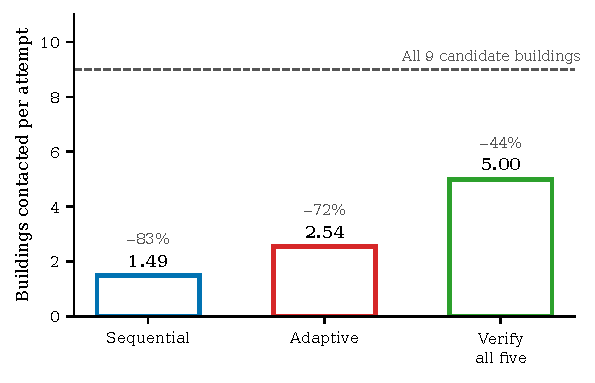
\includegraphics[width=0.5\textwidth]{figures/fig2_results.pdf}
\caption{Buildings contacted per identification attempt for routed visitors at 10 buildings (mean over 20 seeds). The dashed line marks the nine candidate buildings, which is the number contacted without routing; the percentages give the reduction relative to it.}
\label{fig:results}
\end{figure}

\begin{table}[!t]
\caption{Results for routed visitor events at 10 buildings and a shortlist of five (visitors accepted by the capturing building are excluded): mean over 20 seeds with 95\% confidence half-widths ($\pm$). The centralized baseline is a single central endpoint, so no building count is given. Payload is the estimated captured-embedding traffic per attempt.}\label{tab:adaptive}%
\begin{tabular}{@{}lcccc@{}}
\toprule
Method & Correct (\%) & Misidentified (\%) & Buildings & Payload (KB) \\
\midrule
Centralized (450 identities) & $95.50 \pm 0.25$ & $1.31 \pm 0.10$ & -- & 2.0 \\
Sequential & $92.19 \pm 0.28$ & $2.06 \pm 0.12$ & 1.49 & 3.1 \\
Adaptive & $92.95 \pm 0.28$ & $1.30 \pm 0.11$ & 2.54 & 5.2 \\
Verify all five & $92.81 \pm 0.29$ & $1.44 \pm 0.10$ & 5.00 & 10.2 \\
\bottomrule
\end{tabular}
\end{table}

\subsection{Bloom-Filter False-Positive Rate}
\label{sec:fpr}

The Bloom filters are configured for a false-positive probability of 1\%, whereas the effective rate, measured by testing the enrolled items of the other nine buildings against each filter, is $3.54 \pm 0.02\%$. Without a Bloom array, $2.61 \pm 0.02\%$ of the items of other buildings already equal an enrolled item in the same slot, close to the 2.41\% expected if the codes of 50 occupants were evenly distributed over $2^{11}=2048$ values, whereas the Bloom array alone yields $0.94 \pm 0.01\%$ on random integers that were never inserted. The excess over the configured target comes from collisions between the LSH codes of different occupants and not from the Bloom array.

\subsection{Communication Cost}
\label{sec:cost}

The estimates use message sizes and the measured number of buildings contacted, and they exclude protocol headers, replies, filter updates and synchronization. A 512-dimensional float32 embedding occupies 2,048 bytes, so an attempt contacting $q$ buildings generates $2048q$ bytes. Centralized search sends the embedding once to a central endpoint (2.0~KB), which holds all reference embeddings (20.5~MB). The distributed design shares ten Bloom filters of 7.3~KB each (73~KB in total), held by every building. An attempt costs 3.1~KB under sequential verification, 5.2~KB under adaptive verification and 10.2~KB when all five shortlisted buildings are contacted, against 18.4~KB for contacting all nine candidate buildings, and routing requires $(B-1)\cdot L(1+P)=4{,}392$ filter lookups, which grow linearly with the number of buildings.

% ============================================================
% DISCUSSION
% ============================================================

\section{Discussion}
\label{sec:discussion}

The accuracy gap to centralized search has three sources: routing failures (3.78\%, the correct building is not shortlisted), verification failures (1.97\%, the correct building is shortlisted but rejects the identity) and misidentifications (1.44\%, another identity is accepted). Routing failures are the largest, so a more discriminative ranking would help more than a different local verifier. Sequential verification accepts the first building that reaches the vote threshold, so a wrongly ranked building raises misidentification, whereas verifying all five lets the best-voting candidate win at the cost of more contacts. Adaptive verification applies the sequential rule when the top-two score gap exceeds $g_0$ and verifies all shortlisted buildings when the ranking is ambiguous, which lowers misidentification to 1.30\% with 2.54 contacts on average; its gain over verifying all five is small but consistent across seeds. Bloom-filter false positives add candidate matches that local verification may reject, but they can also change the building ranking and the shortlist coverage, so they may affect identification outcomes as well as communication cost. A further 3.3\% of visitors are accepted by the capturing building before routing, an error that routing cannot correct.

From a security perspective, the filters are derived from LSH codes that preserve similarity, so a party with access to them and to the public hash parameters could test whether a given face produces filter hits for a building and infer that the person may be registered there, although no reference embedding is shared. Protecting the filters through access control, keyed hashing or encryption is left for future work.

% ============================================================
% CONCLUSION
% ============================================================

\section{Conclusion}
\label{sec:conclusion}

This work presented a routing mechanism for visitor identification across multiple buildings, in which per-building Bloom filters of LSH codes direct a captured face to the buildings likely to hold the matching reference, without a central database of reference embeddings. The experiments demonstrate the routing and verification of visitors; they do not demonstrate complete occupant tracking, state-transition correctness or formal privacy protection. On 500 CASIA-WebFace identities distributed over 10 buildings, verifying all five shortlisted buildings achieved 92.81\% correct identification for routed visitors against 95.50\% for centralized search, and the adaptive policy achieved 92.95\% while contacting 2.54 of the nine candidate buildings, with an estimated 5.2~KB of captured-embedding payload per attempt. The reduction in contacted buildings is accompanied by a loss of recall when the correct building is not shortlisted, and by a false-positive rate that LSH code collisions raise above the Bloom-filter design value. Future work includes more reliable candidate ranking, protection of the shared filters, unknown visitors, and measured communication costs.

% ============================================================
% LIMITATIONS
% ============================================================

\section{Limitations}
\label{sec:limitations}

The evaluation uses 500 identities from a single public dataset and 10 buildings, and the confidence intervals reflect variation in building assignment, hash randomness and the simulated day rather than a different population. The values $K=11$ and $P=3$ were chosen after observing accuracy on the test images, without a separate validation set, and the overlap between the ArcFace training data and CASIA-WebFace was not checked. The evaluation is closed-set, so unknown individuals were not evaluated, and the 3.3\% of visitors accepted by the capturing building are not recovered by routing. Communication costs are estimated from message sizes, and latency, throughput and filter synchronization were not measured. Encryption and visitor caching were not implemented, no security analysis of the shared filters was carried out, and no formal privacy guarantee is established.

\bmhead{Acknowledgement}

The authors gratefully acknowledge Sri Mata Amritanandamayi Devi (Amma), Chancellor, Amrita Vishwa Vidyapeetham, for her inspiration and for providing financial support for the Article Processing Charges (APC) of this publication.

\bibliography{akd}% akd.bib

\end{document}
